\subsubsection{First touch}




Les résultats de la factorisation et de la résolution triangulaire avec une allocation first touch sur la machine  sont exposés dans le chapitre précèdent.
%
Les résultats ne sont pas aussi bons que ceux que nous pourrions obtenir avec une meilleure gestion de la mémoire.
%


%   (-_-)   %
\begin{figure}[t!]
  \centering
  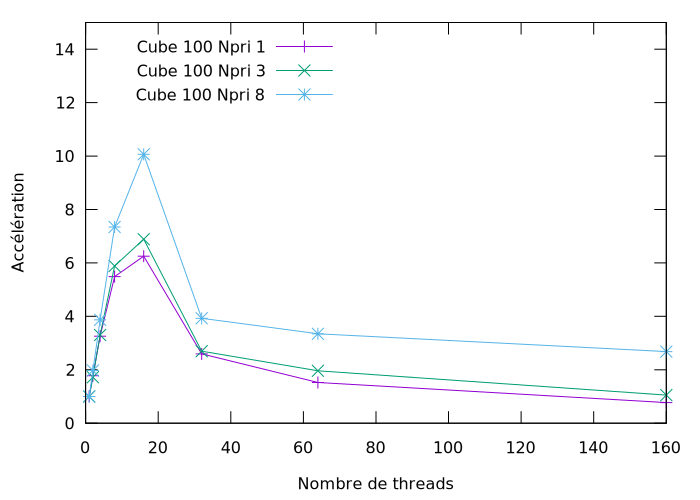
\includegraphics[width=0.7\textwidth]{res_facto_ft_manu}
  \caption{Performance de la factorisation sur Manumanu coeurs en utilisant une politique d'allocation first touch.}
  \label{fig:res_facto_ft_manumanu}
\end{figure}
